\subsection{Etapa de Ideação}


\subsubsection{Backend}

A modelagem do banco de dados sempre será atualizado conforme a necessidade de implementação e conforme forem surgindo as dificuldades de implementação.

\begin{figure}[!htb]
    \centering
    \caption[short]{Modelagem do banco de dados}
    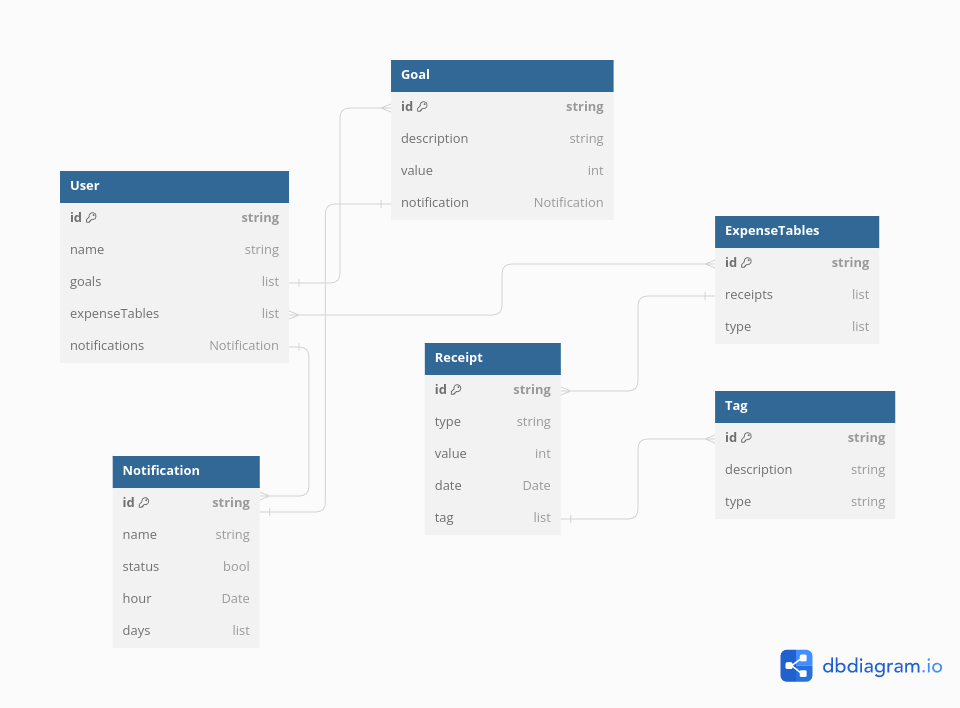
\includegraphics[scale=0.4]{images/backend_model.png}
\end{figure}


\subsubsection{Frontend}

O frontend utilizado foi a partir de um modelo pronto desenvolvido para mobile que será adaptado para uma interface web, visto que um dos requisitos das pessoas entrevistadas era ter uma visão completa de todos os meses, e para isso seria muito melhor ser mostrado dentro de uma tela de computador.

Portanto, todo o design do frontend foi baseado no \textit{Montra}, uma design desenvolvido, especificamente, para mobile.


\noindent{\textit{\textbf{OBS:} O design pode ser observado a partir da figura 3.}}


\subsubsection{Backlog}
\newpage
\begin{longtable}[h!]{ | M{0.5cm} | T{2.7cm} | T{2.7cm} | T{4cm} | l | } \hline

    \textbf{Id} & \textbf{História de Usuário} &\textbf{Regras de Negócio} & \textbf{Critérios de aceite} & \textbf{Prioridade} \\ [5pt] \hline

    1 & Eu como usuário quero adicionar uma nova receita no gerenciamento &O usuário poderá criar quantas receitas achar necessárias para seu gerenciamento & \begin{enumerate}
        \item O usuário deverá criar uma receita por vez
        \item O usuário pode criar quantas receitas forem necessárias.
    \end{enumerate} & Alta \\ \hline


    2 & Eu como usuário quero modificar uma receita existente no gerenciamento & O usuário poderá editar quantas receitas achar necessárias para seu gerenciamento & \begin{enumerate}
        \item O usuário deverá modificar uma receita por vez
        \item O usuário pode modificar quantas receitas forem necessárias.
    \end{enumerate} & Alta \\ \hline


    3 & Eu como usuário quero deletar uma receita no gerenciamento & O usuário poderá deletar quantas receitas achar necessárias para seu gerenciamento & \begin{enumerate}
        \item O usuário deverá deletar uma receita por vez
        \item O usuário pode deletar quantas receitas forem necessárias.
    \end{enumerate} & Alta \\ \hline

    4 & Eu como usuário quero deletar uma despesa no gerenciamento & O usuário poderá deletar quantas despesas achar necessárias para seu gerenciamento & \begin{enumerate}
        \item O usuário deverá deletar uma despesa por vez
        \item O usuário pode deletar quantas despesas forem necessárias.
    \end{enumerate} & Alta \\ \hline

    5 & Eu como usuário quero criar uma despesa no gerenciamento & O usuário poderá criar quantas despesas achar necessárias para seu gerenciamento & \begin{enumerate}
        \item O usuário deverá criar uma despesa por vez
        \item O usuário pode criar quantas despesas forem necessárias.
    \end{enumerate} & Alta \\ \hline

    6 & Eu como usuário quero modificar uma despesa no gerenciamento & O usuário poderá modificar quantas despesas achar necessárias para seu gerenciamento & \begin{enumerate}
        \item O usuário deverá modificar uma despesa por vez
        \item O usuário pode modificar quantas despesas forem necessárias.
    \end{enumerate} & Alta \\ \hline

    7 & Eu como usuário quero visualizar o ano inteiro com todos os gastos e receitas em seus respectivos meses. & O usuário poderá ter a visão anual de gastos e receitas em cada mês. & \begin{enumerate}
        \item O usuário deverá visualizar todos os meses no ano.
        \item O usuário deverá visualizar em cada mês deverá constar cada despesa ou receita respectiva a cada mês.
    \end{enumerate} & Alta \\ \hline

    8 & Eu como usuário quero visualizar o mês o com todos os gastos e receitas. & O usuário poderá ter a visão mensal de gastos e receitas em cada mês. & \begin{enumerate}
        \item O usuário deverá visualizar de um mês do ano.
        \item O usuário deverá visualizar no mês deverá constar cada despesa ou receita respectiva a cada mês.
    \end{enumerate} & Alta \\ \hline

\end{longtable}